\section{Preamp test}
This section will test all requirements on the \gls{preamp} 


\subsection{1}%\label{req:preamp1}}
According to \autoref{req:preamp1}, a test was made to ensure that the \gls{preamp} not change the signal amplitude more than +-1dB between 20 Hz and 20 kHz. A test was made and is descried in \autoref{app:preamp_frequency_response} and the result is as following \autoref{fig:tests:appendix:amplitude}

\begin{figure}[htbp!]
	\centering
		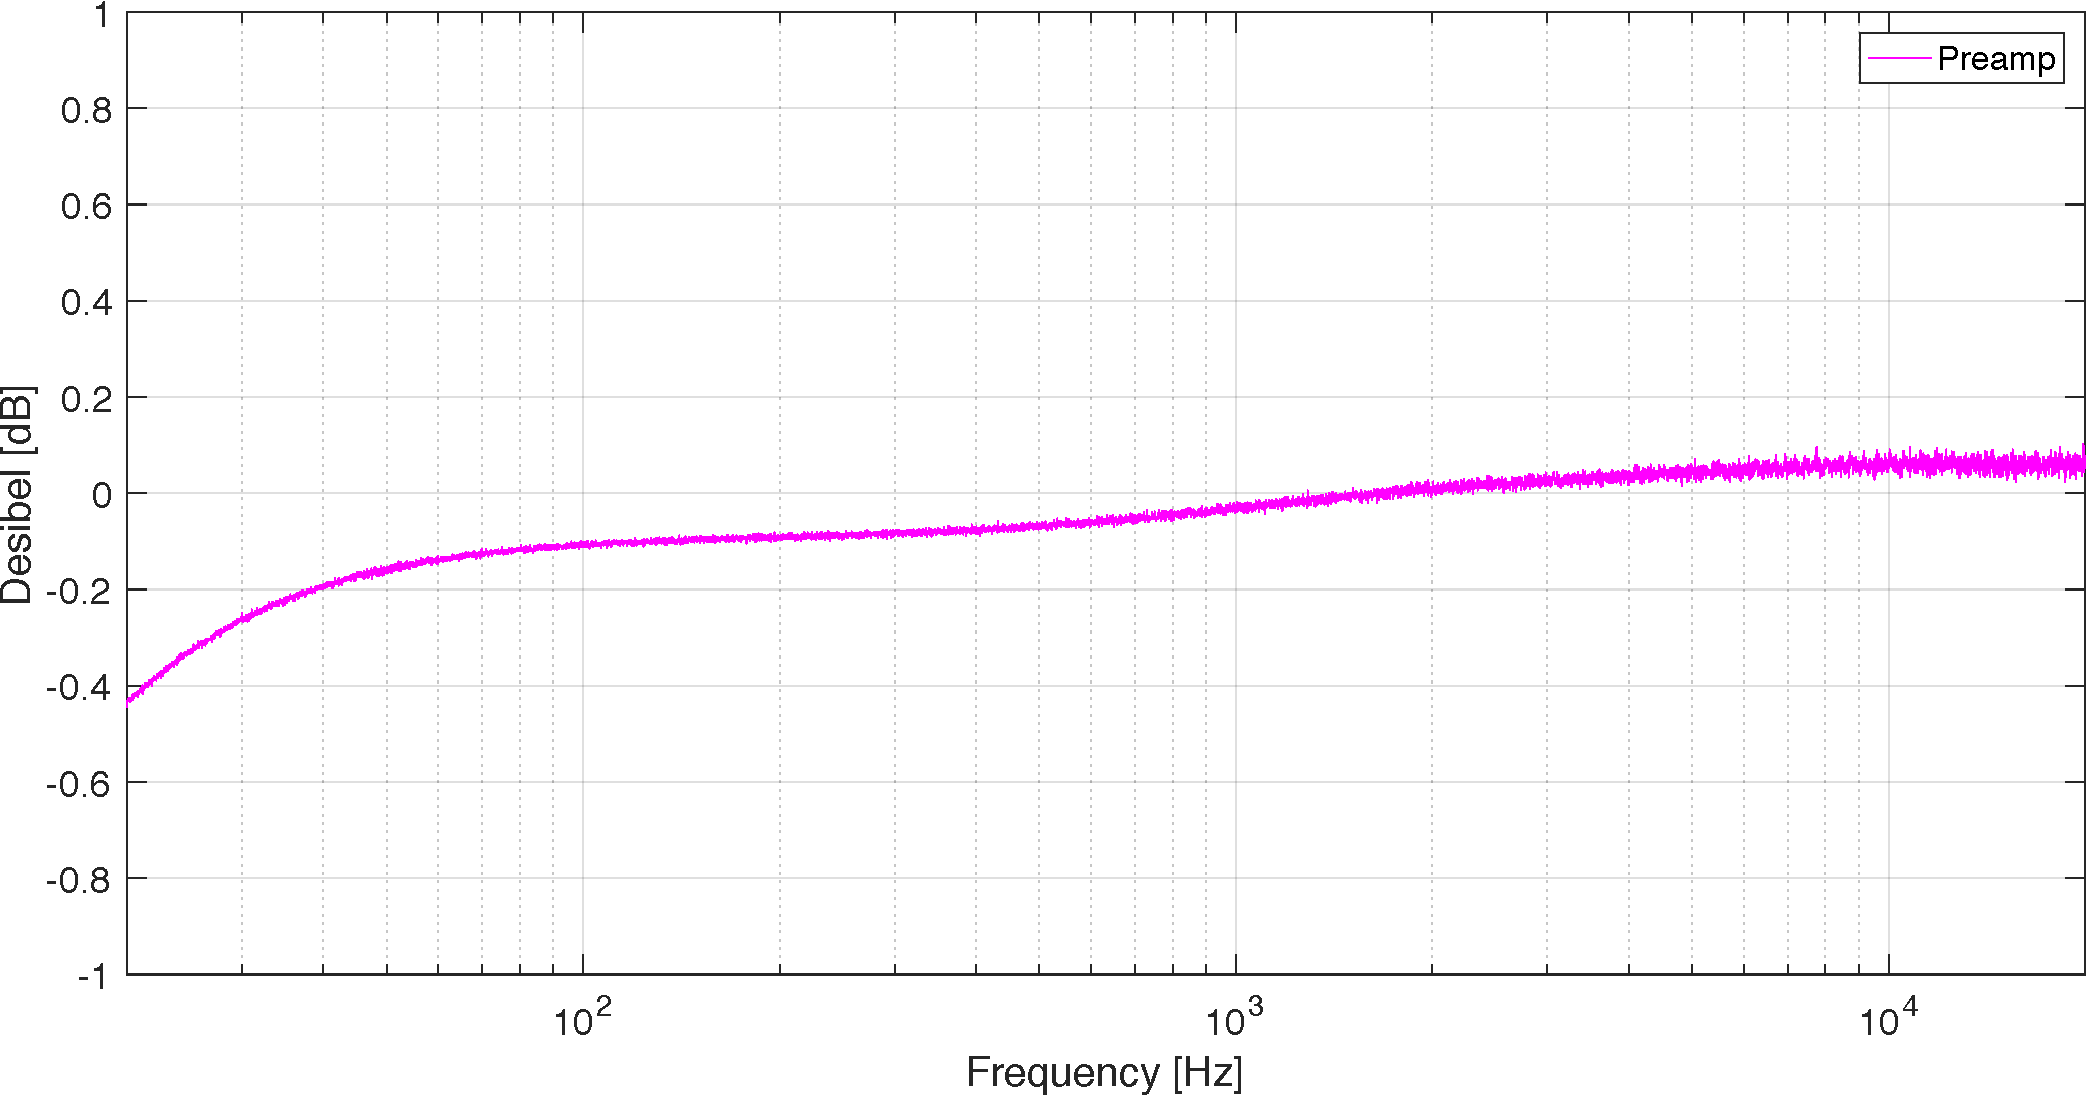
\includegraphics[width=1\textwidth]{preamp_frequency_responce.pdf}
		\caption{Measurement of the real output impedance of the three pickup settings.}
		\label{fig:tests:appendix:amplitude}
\end{figure}

The amplitude is within +-1dB, so \autoref{req:preamp1} is approved

\subsection{2}%\autoref{req:preamp6}}
According to \autoref{req:preamp6}, a test was made to ensure that the \gls{preamp} \gls{pcb} including cable mound fits intro the Jack connector house. The first \autoref{fig:tests:preamp_pcb} shows the \gls{pcb} mounded on the jack connector and the cable is mounted on the \gls{preamp}

\begin{figure}[h]
	\centering
		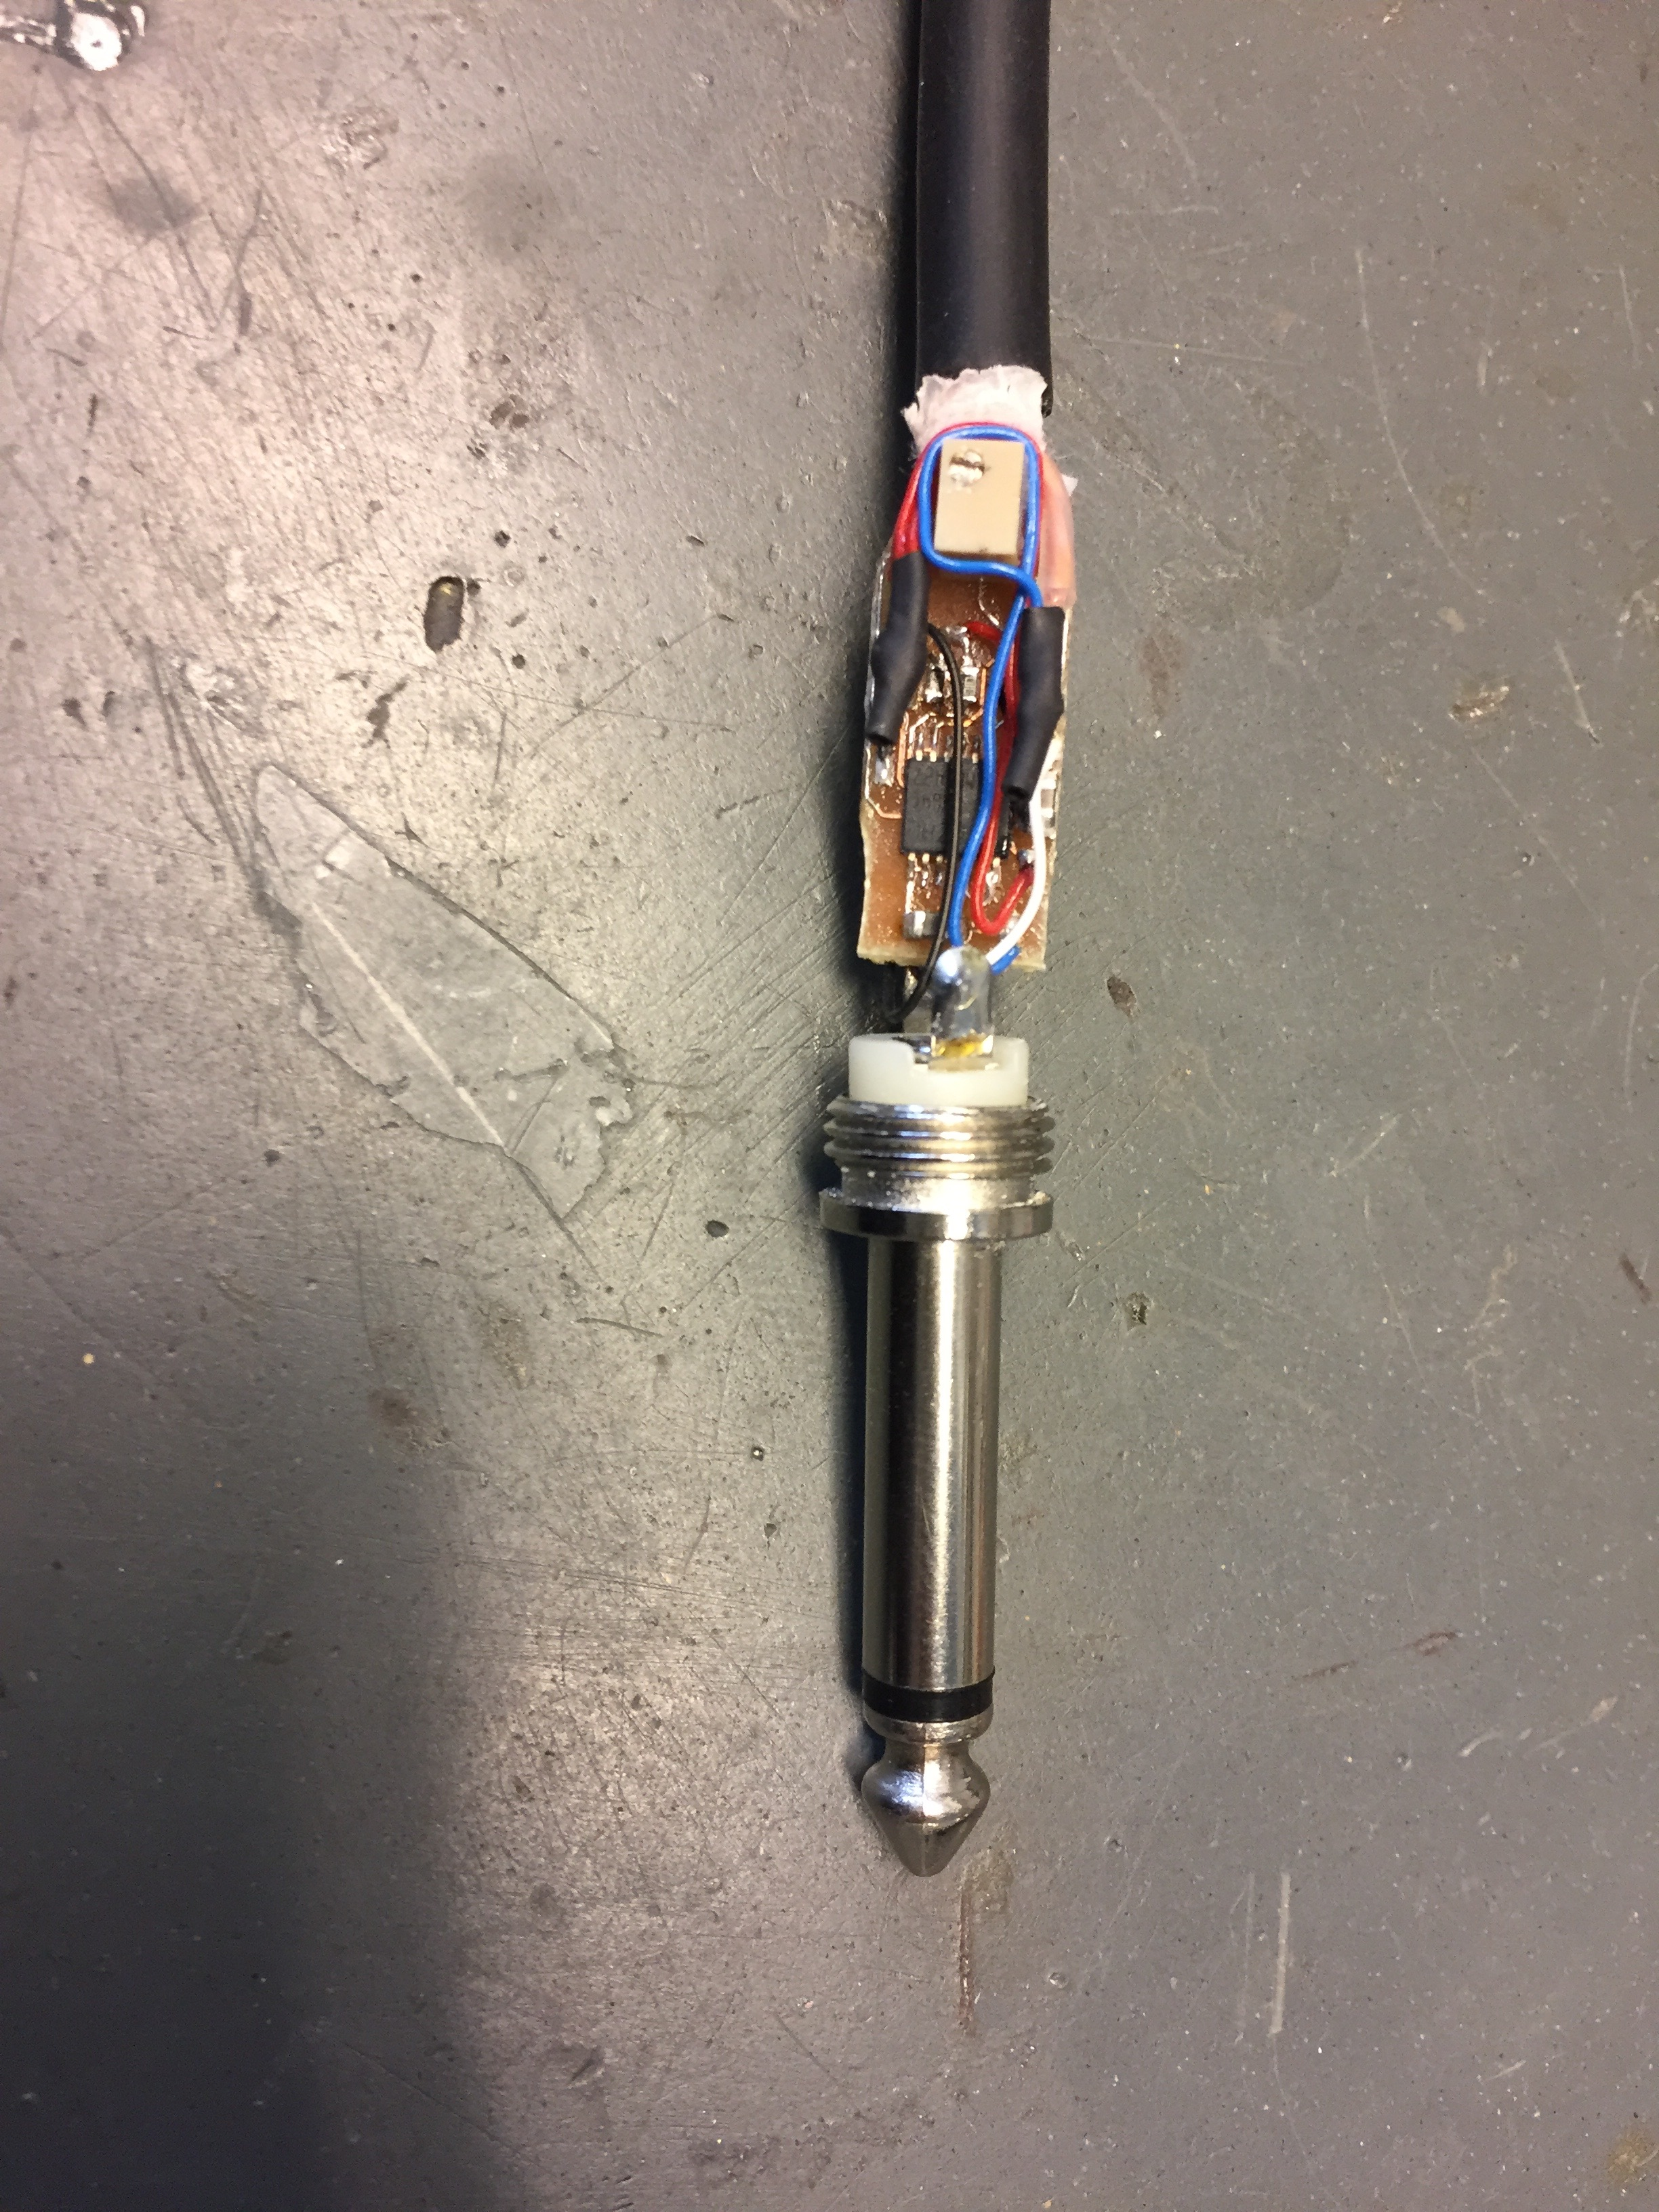
\includegraphics[width=0.4\textwidth , angle=90]{preamp_pcb.jpg}
		\caption{The picture shows the mounted \gls{preamp} \gls{pcb} }
		\label{fig:tests:preamp_pcb}
\end{figure} 

The second \autoref{fig:tests:preamp_jack} shows the \gls{preamp} \gls{pcb} mounted inside the jack connector house.

\begin{figure}[h]
	\centering
		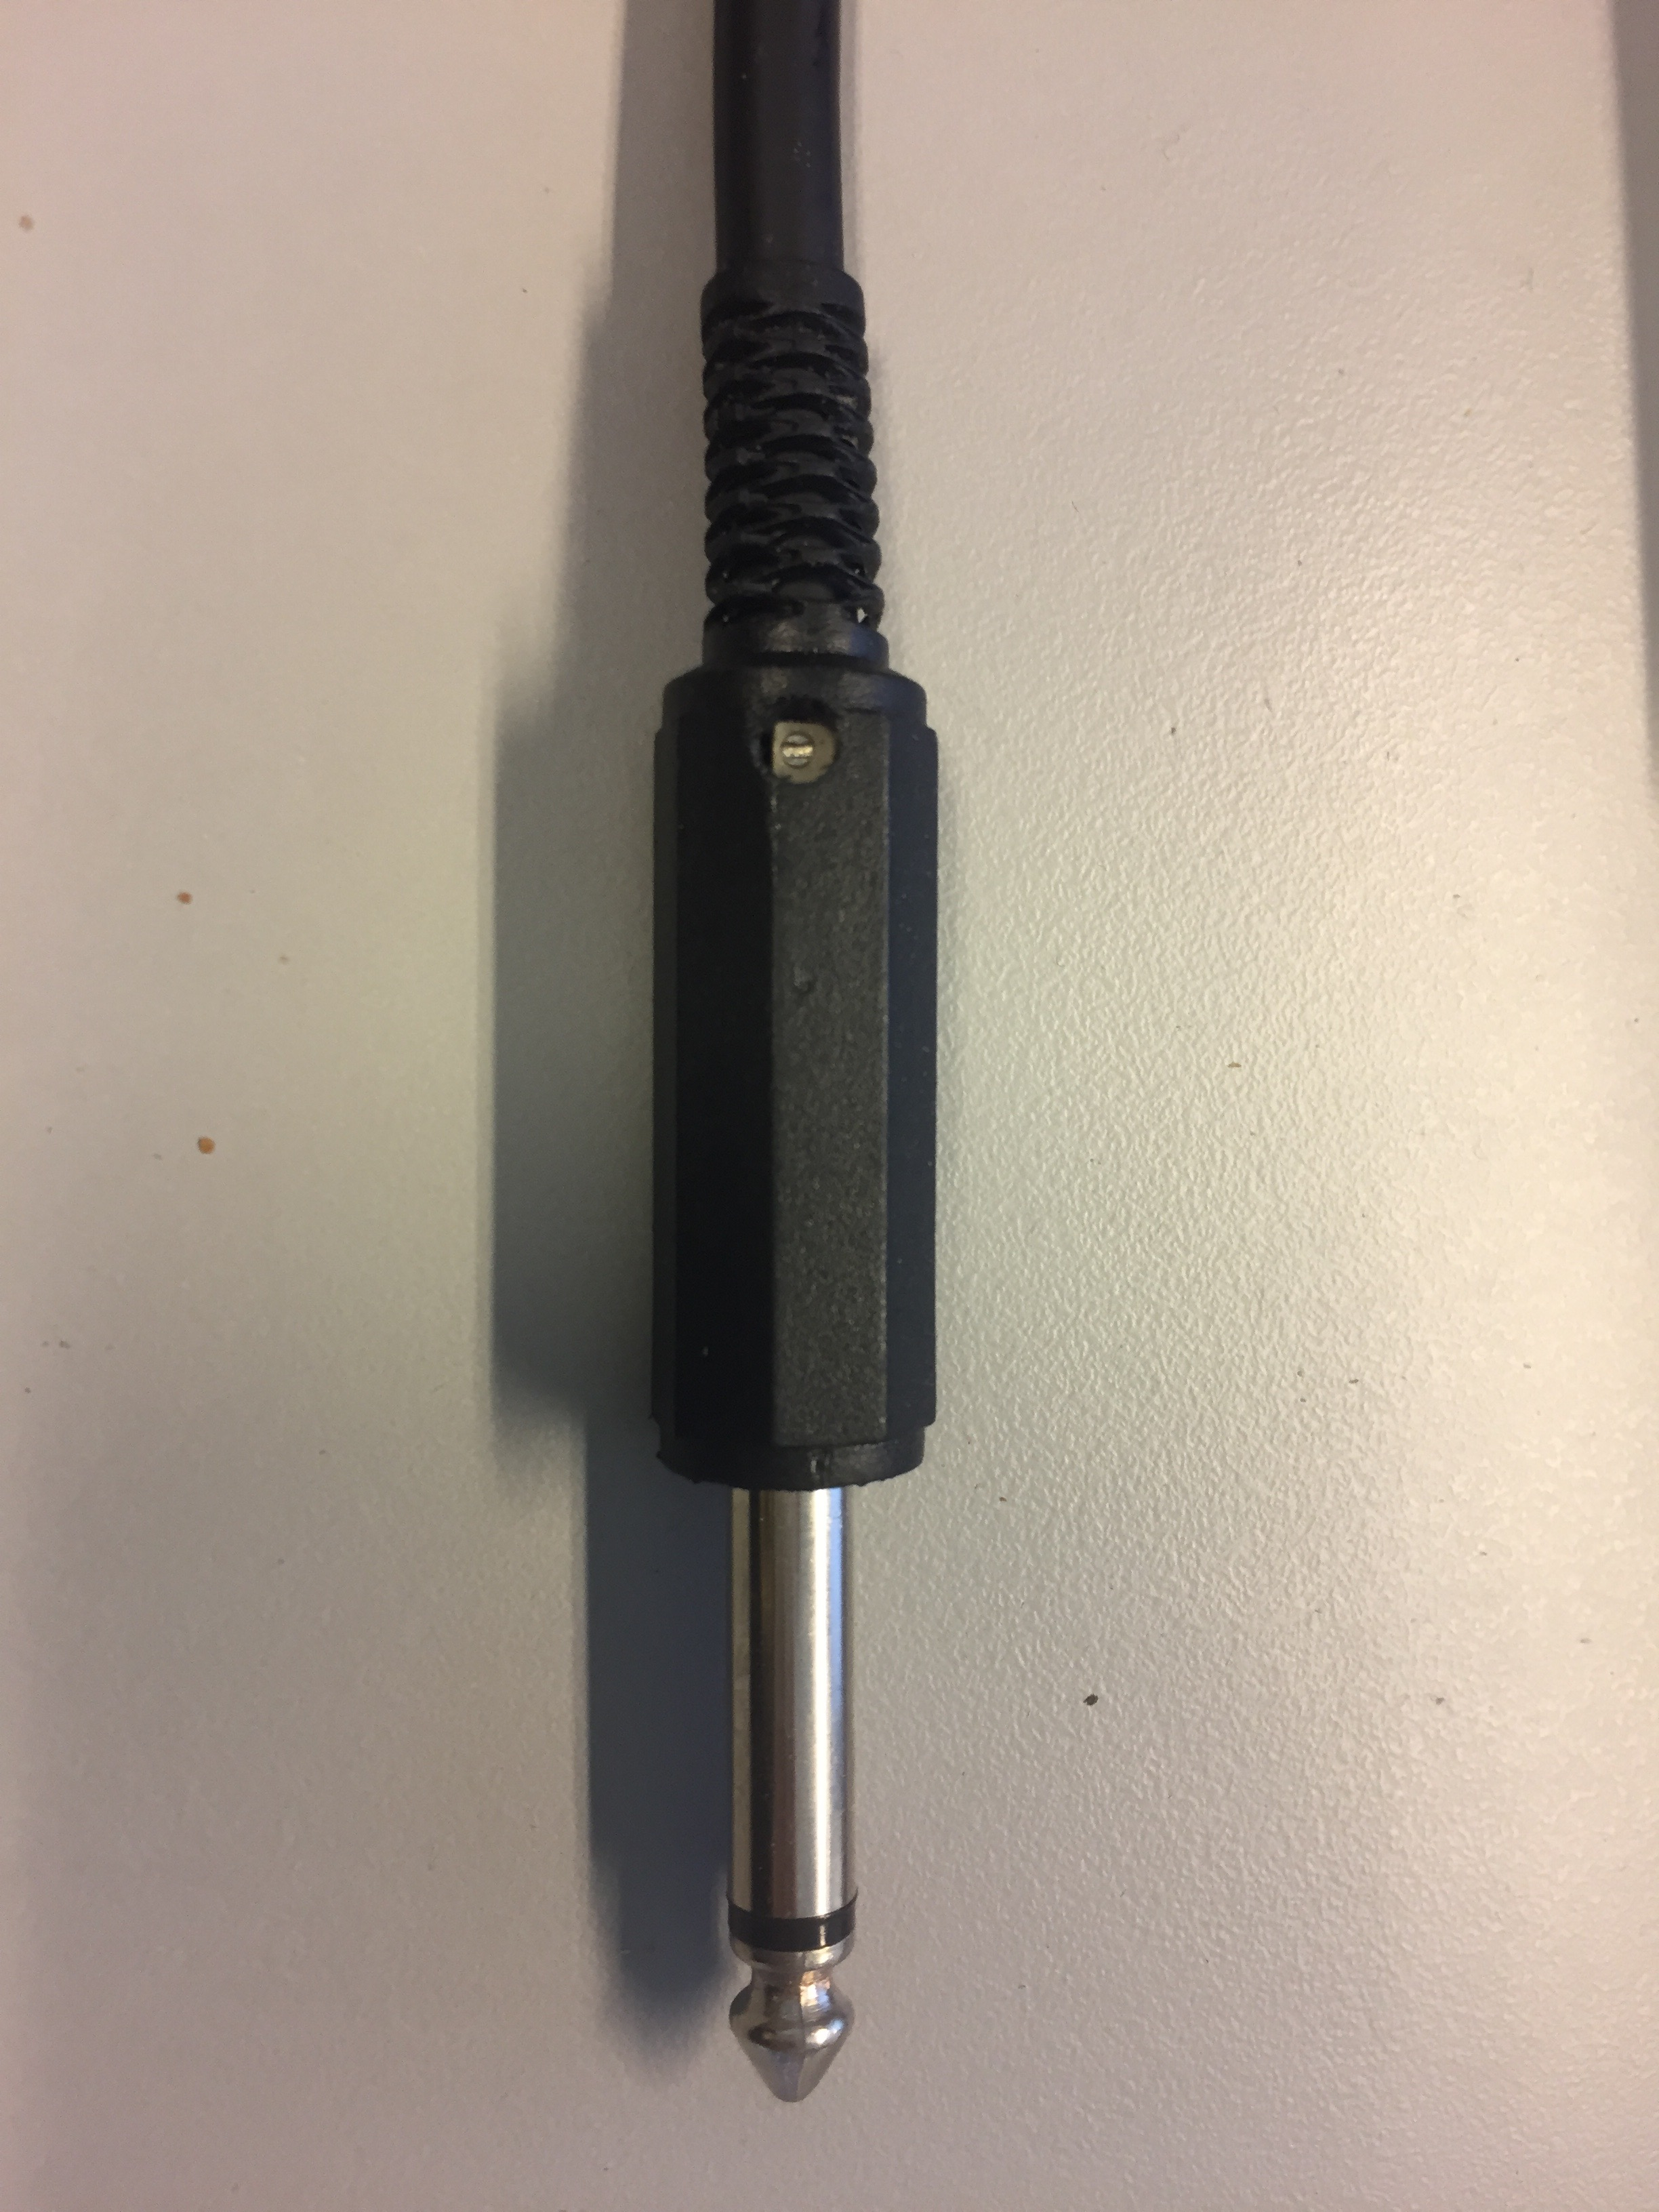
\includegraphics[width=0.4\textwidth , angle=90]{preamp_jack.jpg}
		\caption{The picture shows the mounted \gls{preamp} \gls{pcb} }
		\label{fig:tests:preamp_jack}
\end{figure} 

The \gls{preamp} \gls{pcb} fits inside the jack house, so \autoref{req:preamp6} is approved